\documentclass[10pt,a4paper]{article}
\usepackage{hyperref}
\usepackage{graphicx}
\usepackage{geometry}
\usepackage[utf8]{inputenc}
\usepackage[T1]{fontenc}
\usepackage{doi}
\usepackage[style=apa, sorting=ynt,doi=false]{biblatex}
\usepackage{enumitem}
\usepackage{makecell}
\usepackage{tabularx}
\usepackage{titlesec}

%\usepackage{academicons}
%\usepackage{hanging}
%\usepackage{fontawesome}
%\usepackage{amsmath}


% Structure

\newcommand{\cventry}[4]{
  \begin{tabularx}{\linewidth}{@{}p{1in} X@{}}
  	#1    & \makecell[{{X}}t]{\textbf{#2}, #3\\#4}
  \end{tabularx}\smallskip\smallskip
}


% Layout

\geometry{left=1in,right=1in,top=1in,bottom=1in}
\pagenumbering{gobble}
\setlength{\parindent}{0pt}

\titleformat{\section}
{\normalfont\Large\bfseries}{\thesection}{1em}{}[{\hrule}]

%Preamble

\title{\textsc{Curriculum Vitae}}
\date{}
\addbibresource{publications.bib}

\begin{document}
\maketitle
\begin{minipage}[b]{.7\linewidth}
	\Large \textbf{Arne Van Den Kerchove}\\
	\normalsize Doctoral Researcher Computational Neuroscience\\
	KU Leuven, University of Lille
  \bigskip

  \texttt{arne.vandenkerchove@kuleuven.be \\
  arne.vandenkerchove@univ-lille.fr \\
  arne@vandenkerchove.com \\
  +32 473 32 78 71 \\
	\url{https://arne.vandenkerchove.com}\\
	\url{https://orcid.org/0000-0002-9367-2986} \\
  \url{https://linkedin.com/in/arnevdk} \\}

%	\begin{tabular}{@{}c l}
%		\faAt        & arne.vandenkerchove@kuleuven.be             \\
%		\faAt        & arne.vandenkerchove@univ-lille.fr           \\
%		\faAt        & arne@vandenkerchove.com                     \\
%		\faPhone     & +32 473 32 78 71                            \\
%		\faMapMarker & Leuven, Belgium                             \\
%		\faMapMarker & Laboratory for Neuro- and Psychophysiology  \\
%		             & KU Leuven - Campus Gasthuisberg             \\
%		             & ON II - Herestraat 49 - box 1021            \\
%		             & BE-3000 Leuven                              \\
%		\faMapMarker & UMR CRIStAL                                 \\
%		             & Université de Lille - Campus scientifique   \\
%		             & Bâtiment ESPRIT - Avenue Henri Poincaré     \\
%		             & FR-59655 Villeneuve d'Ascq                  \\
%		\faGlobe     & \url{https://arne.vandenkerchove.com}       \\
%		\aiOrcid     & \url{https://orcid.org/0000-0002-9367-2986} \\
%		\faLinkedin  & \url{https://linkedin.com/in/arnevdk}
%	\end{tabular}
\end{minipage}%
\begin{minipage}[b]{.29\linewidth}
	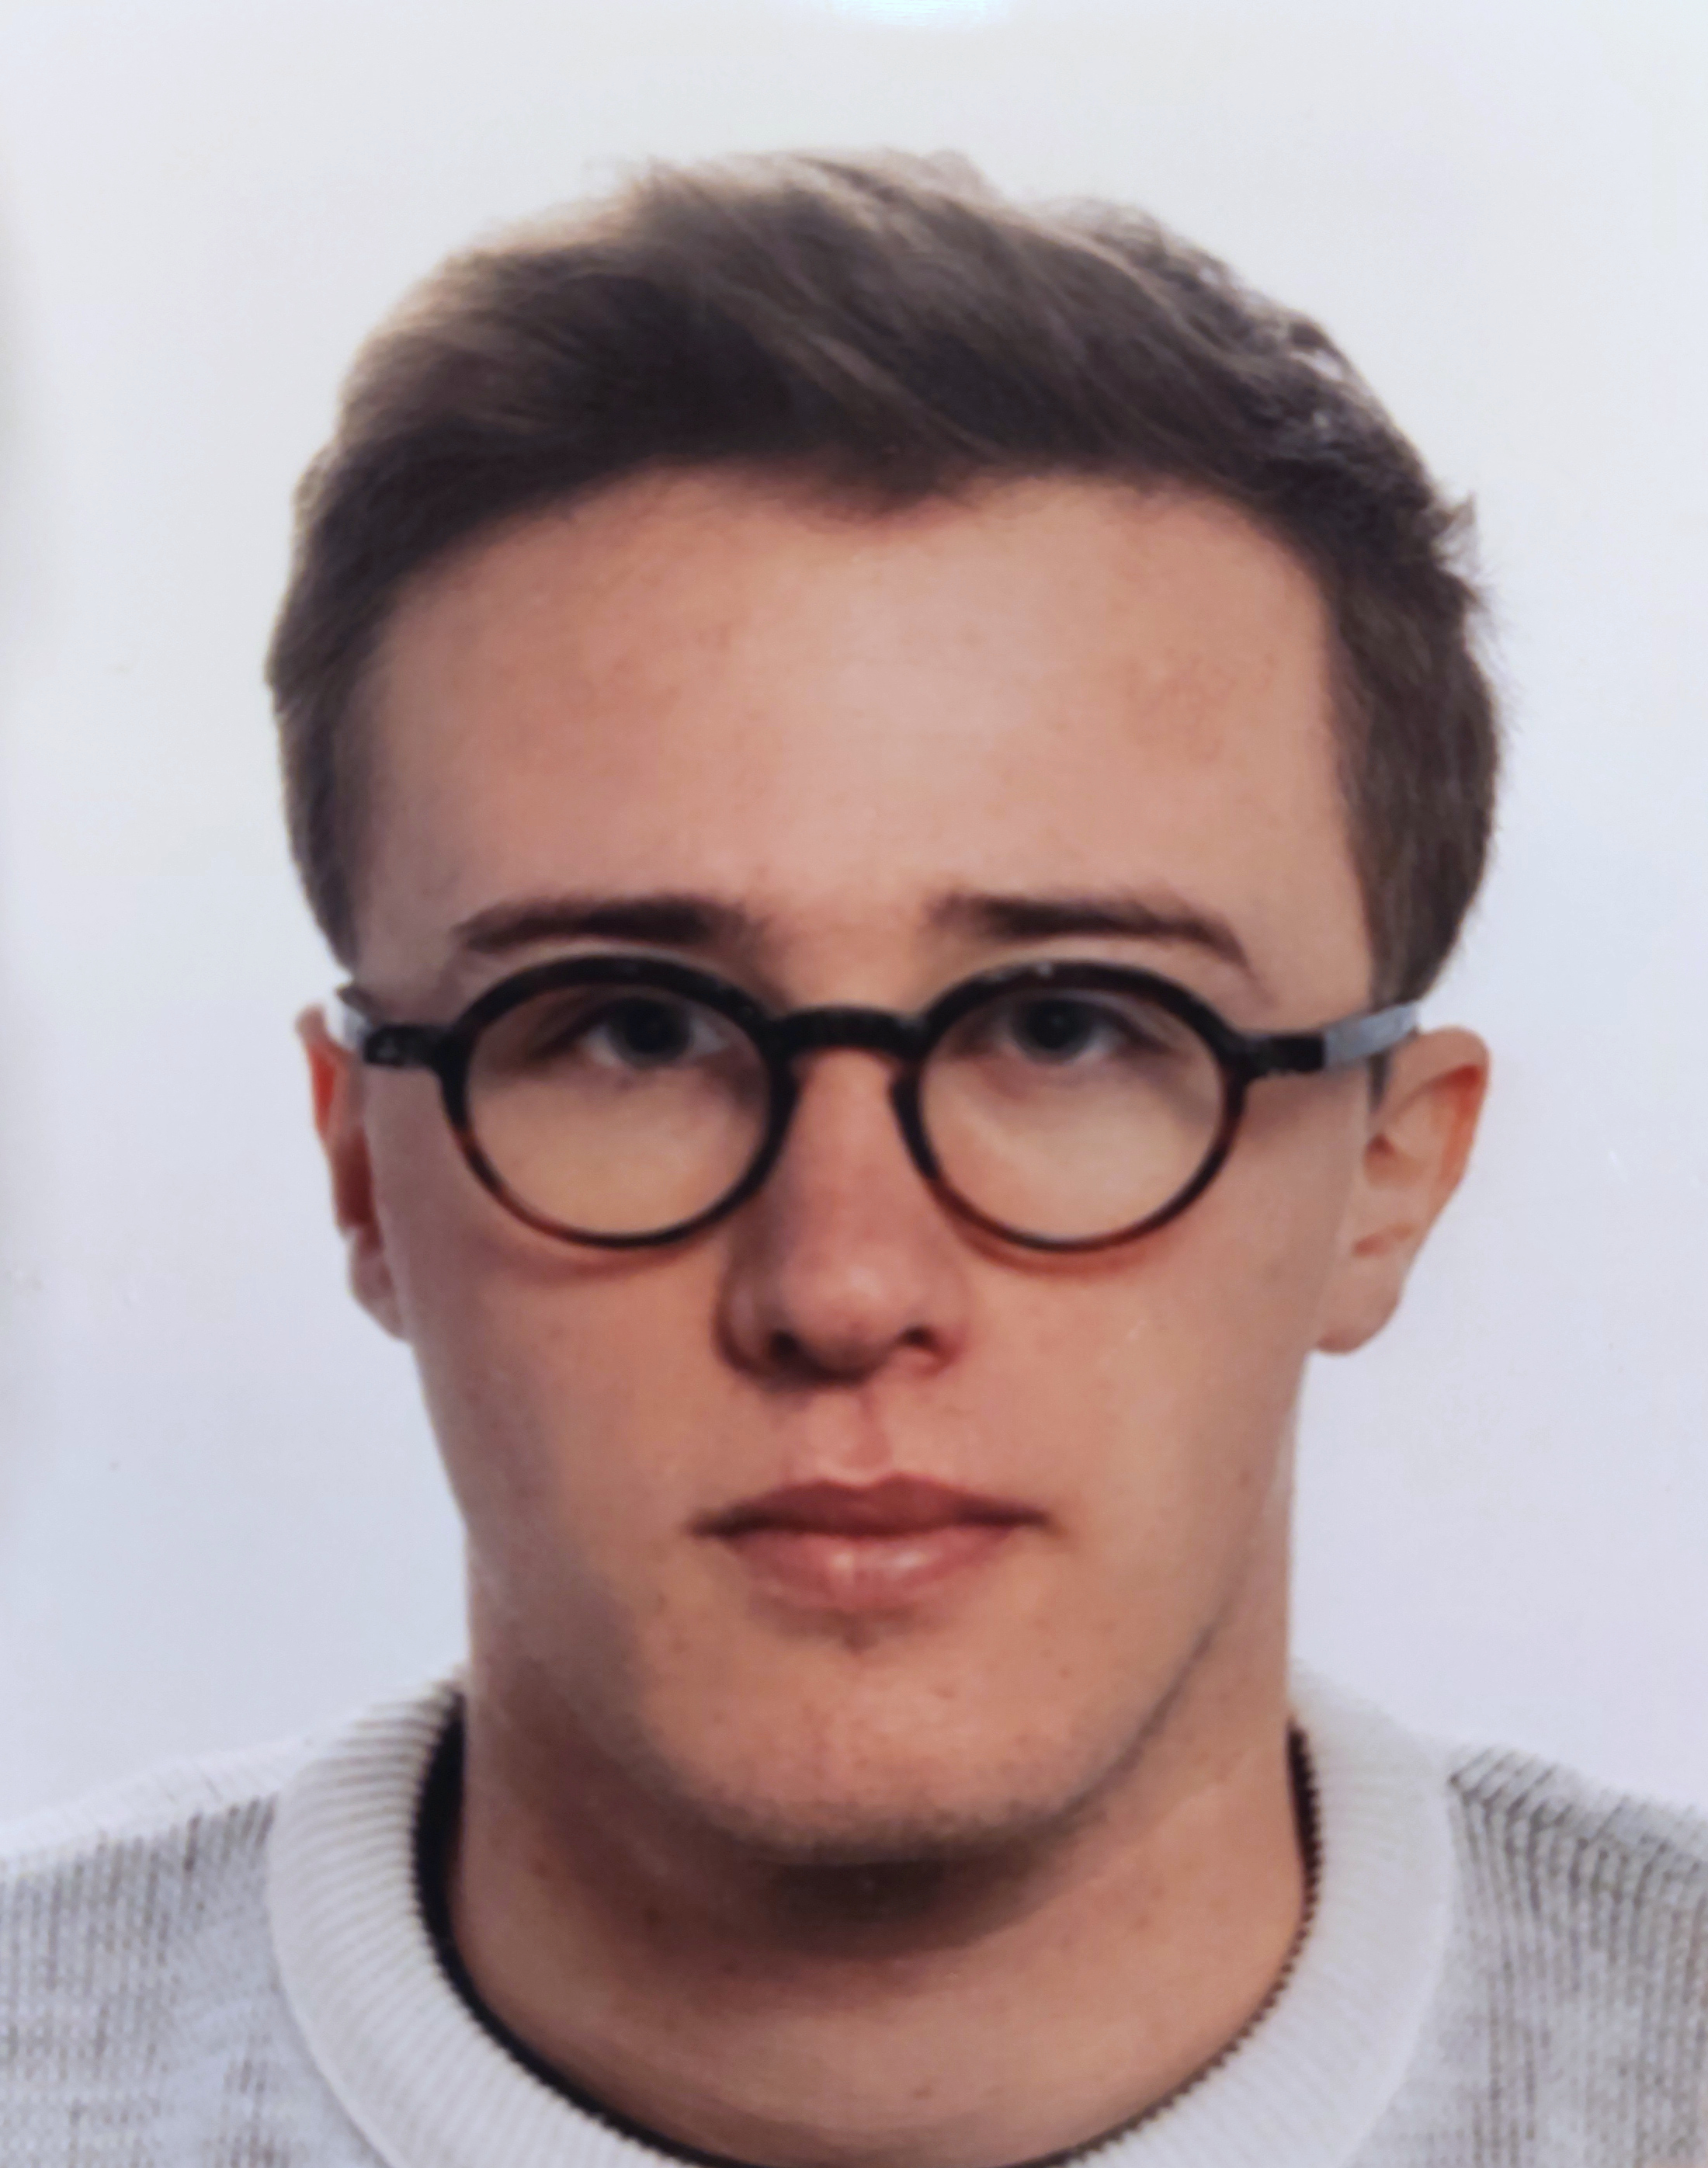
\includegraphics[width=\linewidth]{photo.jpg}
\end{minipage}


\section*{About me}

I am a Ph.D. candidate at KU Leuven Laboratory for Neuro- and Psychophysiology
and the University of Lille Research Center for Informatics, Signal Processing,
and Control Science. My research is centered on developing brain-computer
interface (BCI) technologies with a primary focus on assisting individuals with
severe disabilities, especially those with motor and eye movement impairments.
My goal is to enhance their quality of life by creating accurate and
user-friendly BCIs. Combining my expertise in machine learning, signal
processing, and user interface design with insights from neurophysiology, my
PhD centers around the development of an event-related potential BCI system
using EEG for real-time communication. I strongly believe in the potential of
innovative neurotechnology to empower individuals and patients, enabling them
to lead more independent and fulfilling lives.

\paragraph{Keywords:} brain-computer interfaces, event-related
potentials, multilinear classification, covert visual attention

\section*{Education}

\cventry{ongoing}{Ph.D. in Biomedical Sciences}{KU Leuven}{Supervisor: prof.
  Marc Van Hulle}
\cventry{ongoing}{Ph.D. in Control Science and Signal Processing}{University of
  Lille}{Supervisor: prof. François Cabestaing}
\cventry{2020}{M.Sc. in Engineering Science: Computer Science}{KU Leuven}{
  %Thesis: \textit{Linguistic transcription of EEG responses to sequences of visual stimuli}                \\
  Supervisor: prof. Marc Van Hulle                                                                         \\
  Major: Artificial Intelligence                                                                           \\
  Degree: \textit{cum laude}                                                                               \\
}
\cventry{2017}{B.Sc. in Informatics}{KU Leuven}{
  % Thesis: \textit{Development of a quadcopter simulator and autopilot with stereoscopic object detection} \\
  Minor: Natural Sciences
}

\section*{Publications}

\nocite{*}

\printbibliography[heading=none]


\section*{Awards}

\cventry{2022}{BCI competition 4th place worldwide}{NeuroTechX}{
		Our NeuroTechLeuven BrainBrowsR project, a plug-and-play BCI system that lets you control
    social media applications  trough SSVEP-BCI was awarded 90/100 points by
    the jury of the NeuroTechX international student club competition.
}


\section*{Funding}

\cventry{2021 - 2024}{Global Ph.D. Partnership Grant}{KU Leuven and University
  of Lille}{Topic: \textit{EEG-based visual brain-computer interface for
  gaze-free communication}}


\section*{Conferences and presentations}

\subsection*{Presented}

\cventry{2023}{10th International BCI Meeting}{BCI Society}{
	Poster presentation on classifier-based latency estimation for
	gaze-independent BCIs.}
\cventry{2022}{Leuven.AI Scientific Workshop 2022}{Leuven.AI}{
  Poster presentation on (multi-)Kronecker-structured linear discriminant
	analysis for low sample size event-related potential classification.}
\cventry{2022}{CORTICO 2022}{CORTICO}{
	Oral presentation on Kronecker-structured LCMV-beamforming for event-related potential
	classification.}
\cventry{2021}{CORTICO 2021}{CORTICO}{
	Presentation at CORTICO Young Researchers Day about a multi-component approach
	to spatiotemporal beamforming decoding of event-related potentials.}

\subsection*{Attended}

\cventry{2024}{BCI \& Neurotechnology Spring School 2024}{g.tec}{}
\cventry{2023}{Closed Loop Neurotechnologies Autumn School}{NeurotechEU}{}
\cventry{2023}{CORTICO 2023}{CORTICO}{}
\cventry{2023}{BCI \& Neurotechnology Spring School 2023}{g.tec}{}
\cventry{2022}{BCI \& Neurotechnology Masterclass Belgium}{g.tec}{}
\cventry{2022}{BCI \& Neurotechnology Spring School 2022}{g.tec}{}

\section*{Teaching Experience}

\subsection*{Classes}

\cventry{2022 - ongoing}{Teaching Assistant Brain-Computer Interfaces}{KU
Leuven}{
	Teaching exercise sessions in BCI design and signal processing to students in
  the Master of Bioengineering and Advanced Master of Artificial Intelligence.}
\cventry{2022}{Teaching Assistant Fundamentals of Computer Science}{KU Leuven}{
  Teaching exercise sessions in Python programming and algorithmic reasoning to
  students in the Bachelor of	Engineering Sciences.}

\subsection*{Master theses and internships}

\cventry{2024}{Eye-tracker and ERP data fusion for gaze-independent visual
BCI}{Juliette  Meunier, University of Lille}{}
\cventry{2023 - 2024}{Linear Discriminant Analysis in	the combined
space-time-frequency domain for BCI decoding}{Lunkyadi Sucipto, KU Leuven}{}
\cventry{2023 - 2024}{Tackling the Midas Touch problem in eye tracking with a
BCI}{Reniflal Ebenezer Sundaralal, KU Leuven}{}
\cventry{2023 - 2024}{A connectivity-based EEG  analysis of Alzheimer’s Disease
and Frontotemporal Dementia}{Zoe Barinaga, KU Leuven}{}
\cventry{2023}{Single-trial ERP component latencies as a predictor for the mode
of visual attention}{Yildiz Dilara Parry, KU Leuven}{}
\cventry{2021 - 2022}{A hybrid P300-gaze BCI alternative for navigating virtual
spaces}{Gijs Claes, KU Leuven}{}

\subsection*{Extracurricular}

\cventry{2022 - ongoing}{Project supervisor}{NeuroTech Leuven}{
	Project supervisor and technical advisor for extracurricular
	neurotechnology student projects and a student team competing in the annual NeuroTechX BCI competition.}
\cventry{2015 - 2016}{PAL tutor Principles of Computer Programming}{KU
  Leuven}{ Organizing and teaching peer-assisted learning sessions in Python programming for first year informatics	students.}

\section*{Professional and volunteering Experience}

\cventry{2022 - ongoing}{Ambulance EMT}{Red Cross, FAST	vzw}{}
\cventry{2019}{Python developer}{Mindspeller}{
		Python Flask developer in a KU Leuven spin-off that provides neuromarketing services based on
		scientifically validated neuroscience and AI research.}
    \cventry{2014 - 2020}{Freelance full-stack web developer}{Self-employed}{}
	%2018 - 2019       & \makecell[{{X}}t]{\textbf{Board Secretary}, Scientica Leuven vzw}               \\
	%2015 - 2020       & \makecell[{{X}}t]{\textbf{Webmaster}, Wina Leuven vzw and Scientica Leuven vzw} \\
	%2013 - ongoing    & \makecell[{{X}}t]{\textbf{Event EMT}, Red Cross}                                \\


\section*{Licenses and certifications}
%\begin{tabularx}{\linewidth}{@{}p{1.2in} X@{}}
%	2022 & \makecell[{{X}}t]{\textbf{Ambulance EMT}, FOD
%	Volksgezondheid}                                                 \\
%	2021 & \makecell[{{X}}t]{\textbf{ICH Good Clinical Practice E6},
%	TransCelerate BioPharma Inc. }                                   \\
%\end{tabularx}

\textbf{ICH Good Clinical Practice}, E6 TransCelerate BioPharma Inc.
\smallskip

\textbf{Ambulance EMT}, FOD Volksgezondheid \\

\section*{Languages}
\begin{tabularx}{\linewidth}{@{}p{1.2in} X@{}}
	Dutch   & Native           \\
	English & Fully proficient \\
	French  & Advanced         \\
	German  & Intermediate     \\
\end{tabularx}




\end{document}
